\begin{equation}
    \frac{1}{2\pi i}\oint_{\gamma} \frac{f(z)}{z-z_0} \,dz = \sum_{n=0}^{\infty} \frac{f^{(n)}(z_0)}{n!}(z-z_0)^n\label{eq:equation}
\end{equation}

Текст статьи.
Пример цитирования~\cite{kolmogorov1950osnovnye, kolmogorov83kobminatorniye, GithubSource_2022, Sloane_theencyclopedia}.
Lorem ipsum – псевдо-латинский текст, который используется для веб дизайна, типографии, оборудования,
и распечатки вместо английского текста для того, чтобы сделать ударение не на содержание,
а на элементы дизайна.
Такой текст также называется как заполнитель.
Это очень удобный инструмент для моделей (макетов).
Он помогает выделить визуальные элементы в документе или презентации, например текст, шрифт или разметка.
Lorem ipsum по большей части является элементом латинского текста классического автора и философа Цицерона.
Слова и буквы были заменены добавлением или сокращением элементов, поэтому будет совсем неразумно пытаться передать содержание;
это не гениально, не правильно, используется даже не понятный латинский.
Хотя Lorem ipsum напоминает классический латинский, вы не найдете никакого смысла в сказанном.
Поскольку текст Цицерона не содержит буквы K, W, или Z, что чуждо для латинского, эти буквы, а также многие другие
часто вставлены в случайном порядке, чтобы скопировать тексты различных Европейских языков, поскольку диграфы
не встречаются в оригинальных текстах.

В профессиональной сфере часто случается так, что личные или корпоративные клиенты заказывают, чтобы публикация была
сделана и представлена еще тогда, когда фактическое содержание все еще не готово.
Вспомните новостные блоги, где информация публикуется каждый час в живом порядке.
Тем не менее, читатели склонны к тому, чтобы быть отвлеченными доступным контентом, скажем, любым текстом, который
был скопирован из газеты или интернета.
Они предпочитают сконцентрироваться на тексте, пренебрегая разметкой и ее элементами.
К тому же, случайный текст подвергается риску быть неумышленно смешным или оскорбительным,
что является неприемлемым риском в корпоративной среде.
Lorem ipsum, а также ее многие варианты были использованы в работе начиная с 1960-ых, и очень даже похоже,
что еще с 16-го века.

Пример изображения
\begin{figure}[H]
    \centering
    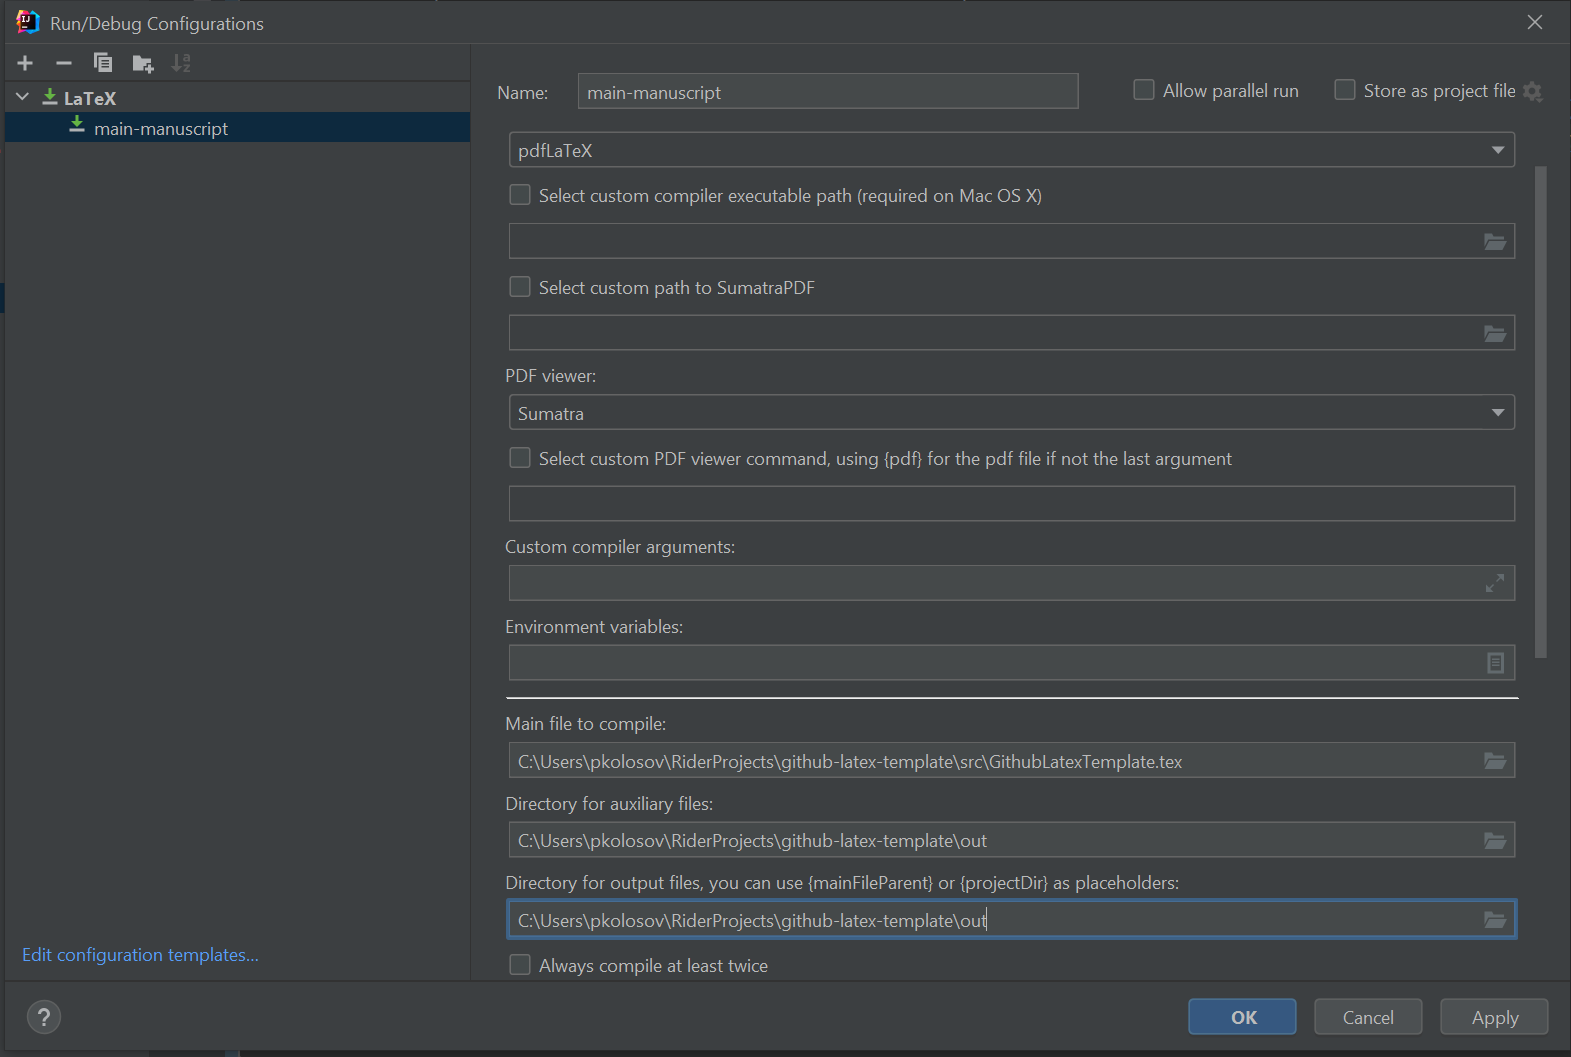
\includegraphics[width=0.8\textwidth]{../img/latex_configuration}
    ~\caption{Пример изображения.}\label{fig:figure}
\end{figure}